\chapter{Supplementary Data} \label{app:supplementary_data}
This section contains some additional tables and figures that did not fit to the main text.

\section*{Generated Speech Datasets} \label{app:sec:generated_speech_datasets}
The \textit{Phonemes} classification problem from \cref{sec:example_speech} works with data that are acquired based on three parameters (\textit{bs}: border size, \textit{cs}: context size and \textit{ns}: number of samples per class). \cref{tab:app:speech_datasets} lists all generated datasets differing in those parameters. For big $ ns $ and/or $ bs $, it might happen that some phonemes are not present in sufficient quantity in the source recordings, therefore those classes are incomplete (e.g. class \texttt{"F"}).

\begin{footnotesize}
\begin{longtable}{|c|c|c|c|c|c|c|c|c|}
\hline
\textit{id} & \textit{bs} & \textit{cs} & \textit{ns} & \textit{incomplete classes} & \textit{total} & \textit{train} & \textit{devel} & \textit{test} \\ \hline
\endhead
ds\_00      & 0           & 0           & 1K        & F (683)                     & 39683         & 31747          & 3968           & 3968          \\ \hline
ds\_01      & 0           & 1           & 1K        & F (683)                     & 39683         & 31747          & 3968           & 3968          \\ \hline
ds\_02      & 0           & 2           & 1K        & F (683)                     & 39683         & 31747          & 3968           & 3968          \\ \hline
ds\_03      & 0           & 3           & 1K        & F (683)                     & 39683         & 31747          & 3968           & 3968          \\ \hline
ds\_04      & 0           & 4           & 1K        & F (683)                     & 39683         & 31747          & 3968           & 3968          \\ \hline
ds\_05      & 0           & 5           & 1K        & F (683)                     & 39683         & 31747          & 3968           & 3968          \\ \hline
ds\_06      & 0           & 6           & 1K        & F (683)                     & 39683         & 31747          & 3968           & 3968          \\ \hline
ds\_07      & 0           & 7           & 1K        & F (683)                     & 39683         & 31747          & 3968           & 3968          \\ \hline
ds\_08      & 0           & 8           & 1K        & F (683)                     & 39683         & 31747          & 3968           & 3968          \\ \hline
ds\_09      & 0           & 9           & 1K        & F (683)                     & 39683         & 31747          & 3968           & 3968          \\ \hline
ds\_10      & 1           & 0           & 1K        & F (589)                     & 39589         & 31672          & 3959           & 3958          \\ \hline
ds\_11      & 1           & 1           & 1K        & F (589)                     & 39589         & 31672          & 3959           & 3958          \\ \hline
ds\_12      & 1           & 2           & 1K        & F (589)                     & 39589         & 31672          & 3959           & 3958          \\ \hline
ds\_13      & 1           & 3           & 1K        & F (589)                     & 39589         & 31672          & 3959           & 3958          \\ \hline
ds\_14      & 1           & 4           & 1K        & F (589)                     & 39589         & 31672          & 3959           & 3958          \\ \hline
ds\_15      & 1           & 5           & 1K        & F (589)                     & 39589         & 31672          & 3959           & 3958          \\ \hline
ds\_16      & 1           & 6           & 1K        & F (589)                     & 39589         & 31672          & 3959           & 3958          \\ \hline
ds\_17      & 1           & 7           & 1K        & F (589)                     & 39589         & 31672          & 3959           & 3958          \\ \hline
ds\_18      & 1           & 8           & 1K        & F (589)                     & 39589         & 31672          & 3959           & 3958          \\ \hline
ds\_19      & 1           & 9           & 1K        & F (589)                     & 39589         & 31672          & 3959           & 3958          \\ \hline
ds\_20      & 2           & 0           & 1K        & F (498)                     & 39498         & 31599          & 3950           & 3949          \\ \hline
ds\_21      & 2           & 1           & 1K        & F (498)                     & 39498         & 31599          & 3950           & 3949          \\ \hline
ds\_22      & 2           & 2           & 1K        & F (498)                     & 39498         & 31599          & 3950           & 3949          \\ \hline
ds\_23      & 2           & 3           & 1K        & F (498)                     & 39498         & 31599          & 3950           & 3949          \\ \hline
ds\_24      & 2           & 4           & 1K        & F (498)                     & 39498         & 31599          & 3950           & 3949          \\ \hline
ds\_25      & 2           & 5           & 1K        & F (498)                     & 39498         & 31599          & 3950           & 3949          \\ \hline
ds\_26      & 2           & 6           & 1K        & F (498)                     & 39498         & 31599          & 3950           & 3949          \\ \hline
ds\_27      & 2           & 7           & 1K        & F (498)                     & 39498         & 31599          & 3950           & 3949          \\ \hline
ds\_28      & 2           & 8           & 1K        & F (498)                     & 39498         & 31599          & 3950           & 3949          \\ \hline
ds\_29      & 2           & 9           & 1K        & F (498)                     & 39498         & 31599          & 3950           & 3949          \\ \hline
ds\_30      & 3           & 0           & 1K        & F (410)                     & 39410         & 31528          & 3941           & 3941          \\ \hline
ds\_31      & 3           & 1           & 1K        & F (410)                     & 39410         & 31528          & 3941           & 3941          \\ \hline
ds\_32      & 3           & 2           & 1K        & F (410)                     & 39410         & 31528          & 3941           & 3941          \\ \hline
ds\_33      & 3           & 3           & 1K        & F (410)                     & 39410         & 31528          & 3941           & 3941          \\ \hline
ds\_34      & 3           & 4           & 1K        & F (410)                     & 39410         & 31528          & 3941           & 3941          \\ \hline
ds\_35      & 3           & 5           & 1K        & F (410)                     & 39410         & 31528          & 3941           & 3941          \\ \hline
ds\_36      & 3           & 6           & 1K        & F (410)                     & 39410         & 31528          & 3941           & 3941          \\ \hline
ds\_37      & 3           & 7           & 1K        & F (410)                     & 39410         & 31528          & 3941           & 3941          \\ \hline
ds\_38      & 3           & 8           & 1K        & F (410)                     & 39410         & 31528          & 3941           & 3941          \\ \hline
ds\_39      & 3           & 9           & 1K        & F (410)                     & 39410         & 31528          & 3941           & 3941          \\ \hline
ds\_40      & 4           & 0           & 1K        & F (327)                     & 39327         & 31462          & 3933           & 3932          \\ \hline
ds\_41      & 4           & 1           & 1K        & F (327)                     & 39327         & 31462          & 3933           & 3932          \\ \hline
ds\_42      & 4           & 2           & 1K        & F (327)                     & 39327         & 31462          & 3933           & 3932          \\ \hline
ds\_43      & 4           & 3           & 1K        & F (327)                     & 39327         & 31462          & 3933           & 3932          \\ \hline
ds\_44      & 4           & 4           & 1K        & F (327)                     & 39327         & 31462          & 3933           & 3932          \\ \hline
ds\_45      & 4           & 5           & 1K        & F (327)                     & 39327         & 31462          & 3933           & 3932          \\ \hline
ds\_46      & 4           & 6           & 1K        & F (327)                     & 39327         & 31462          & 3933           & 3932          \\ \hline
ds\_47      & 4           & 7           & 1K        & F (327)                     & 39327         & 31462          & 3933           & 3932          \\ \hline
ds\_48      & 4           & 8           & 1K        & F (327)                     & 39327         & 31462          & 3933           & 3932          \\ \hline
ds\_49      & 4           & 9           & 1K        & F (327)                     & 39327         & 31462          & 3933           & 3932          \\ \hline
ds\_50      & 5           & 0           & 1K        & F (253)                     & 39253         & 31403          & 3925           & 3925          \\ \hline
ds\_60      & 6           & 0           & 1K        & \begin{tabular}{@{}c@{}}D, F, N, \\ Q, R, T\end{tabular}             
																					& 38049         & 30441          & 3805           & 3803          \\ \hline
ds\_70      & 7           & 0           & 1K        & \begin{tabular}{@{}c@{}}D, F, N, \\ Q, R, T, Z\end{tabular}
																		            & 36140         & 28914          & 3614           & 3612          \\ \hline
ds\_80      & 8           & 0           & 1K        & \begin{tabular}{@{}c@{}}D, F, N, \\ Q, R, T, Z\end{tabular}
																		            & 34869         & 27899          & 3487           & 3483          \\ \hline
ds\_90      & 9           & 0           & 1K        &  \begin{tabular}{@{}c@{}}D, F, N, Q, \\ R, T, Z, b\end{tabular}      
																				    & 33680         & 26947          & 3368           & 3365          \\ \hline
ds\_5K      & 3           & 3           & 5K        &  \begin{tabular}{@{}c@{}}D, F, N, Q, R, \\ T, Y, Z, g\end{tabular}   
																					& 184750        & 147803         & 18475          & 18472          \\ \hline
ds\_10K      & 3           & 3           & 10K      & \begin{tabular}{@{}c@{}}D, F, N, Q, R, \\ T, U, Y, Z, g, x\end{tabular}   
																					 & 335812    & 268654         & 33581          & 33577          \\ \hline
\caption{Generated datasets: \textit{Phonemes} problem.} \label{tab:app:speech_datasets} \\
\end{longtable}
\end{footnotesize}

%\section*{Finding Speech Dataset Params - complete results} \label{app:sec:finding_speech_dataset_parameters}
%
%\begin{longtable}{|c|c|c|c|c|c|c|c|}
%\hline
%\textit{dataset id} & \textit{job 1} & \textit{job 2} & \textit{job 3} & \textit{job 4} & \textit{job 5} & \textit{mean} & \textit{std}\\ \hline
%\endhead
%ds\_00	& 0.0112	& 0.0113	& 0.0117	& 0.0114	& 0.0114	& 0.0114	& 0.0002	\\ \hline
%ds\_01	& 0.0116	& 0.0116	& 0.0114	& 0.0116	& 0.0115	& 0.0115	& 0.0001	\\ \hline
%ds\_02	& 0.0114	& 0.0115	& 0.0114	& 0.0115	& 0.0116	& 0.0115	& 0.0	\\ \hline
%ds\_03	& 0.0116	& 0.0114	& 0.0115	& 0.0118	& 0.0117	& 0.0116	& 0.0001	\\ \hline
%ds\_04	& 0.0117	& 0.0117	& 0.0119	& 0.0117	& 0.0121	& 0.0118	& 0.0002	\\ \hline
%ds\_05	& 0.0116	& 0.0118	& 0.0117	& 0.0116	& 0.0117	& 0.0117	& 0.0001	\\ \hline
%ds\_06	& 0.0118	& 0.0119	& 0.0116	& 0.0118	& 0.0117	& 0.0118	& 0.0001	\\ \hline
%ds\_07	& 0.0118	& 0.0117	& 0.012	& 0.0118	& 0.0119	& 0.0118	& 0.0001	\\ \hline
%ds\_08	& 0.012	& 0.0121	& 0.0116	& 0.0118	& 0.012	& 0.0119	& 0.0002	\\ \hline
%ds\_09	& 0.012	& 0.0119	& 0.0119	& 0.0119	& 0.0119	& 0.0119	& 0.0	\\ \hline
%ds\_00	& 0.0112	& 0.0113	& 0.0117	& 0.0114	& 0.0114	& 0.0114	& 0.0002	\\ \hline
%ds\_01	& 0.0116	& 0.0116	& 0.0114	& 0.0116	& 0.0115	& 0.0115	& 0.0001	\\ \hline
%ds\_02	& 0.0114	& 0.0115	& 0.0114	& 0.0115	& 0.0116	& 0.0115	& 0.0	\\ \hline
%ds\_03	& 0.0116	& 0.0114	& 0.0115	& 0.0118	& 0.0117	& 0.0116	& 0.0001	\\ \hline
%ds\_04	& 0.0117	& 0.0117	& 0.0119	& 0.0117	& 0.0121	& 0.0118	& 0.0002	\\ \hline
%ds\_05	& 0.0116	& 0.0118	& 0.0117	& 0.0116	& 0.0117	& 0.0117	& 0.0001	\\ \hline
%ds\_06	& 0.0118	& 0.0119	& 0.0116	& 0.0118	& 0.0117	& 0.0118	& 0.0001	\\ \hline
%ds\_07	& 0.0118	& 0.0117	& 0.012	& 0.0118	& 0.0119	& 0.0118	& 0.0001	\\ \hline
%ds\_08	& 0.012	& 0.0121	& 0.0116	& 0.0118	& 0.012	& 0.0119	& 0.0002	\\ \hline
%ds\_09	& 0.012	& 0.0119	& 0.0119	& 0.0119	& 0.0119	& 0.0119	& 0.0	\\ \hline
%ds\_10	& 0.0114	& 0.0114	& 0.0112	& 0.0113	& 0.0114	& 0.0113	& 0.0001	\\ \hline
%ds\_11	& 0.0114	& 0.0115	& 0.0115	& 0.0111	& 0.0117	& 0.0115	& 0.0002	\\ \hline
%ds\_12	& 0.0113	& 0.0115	& 0.0113	& 0.0114	& 0.011	& 0.0113	& 0.0002	\\ \hline
%ds\_13	& 0.0115	& 0.0115	& 0.0116	& 0.0114	& 0.0117	& 0.0115	& 0.0001	\\ \hline
%ds\_14	& 0.0118	& 0.0115	& 0.0115	& 0.0113	& 0.0116	& 0.0115	& 0.0002	\\ \hline
%ds\_15	& 0.0116	& 0.0119	& 0.0119	& 0.0116	& 0.0115	& 0.0117	& 0.0002	\\ \hline
%ds\_16	& 0.0117	& 0.012	& 0.0118	& 0.0112	& 0.0118	& 0.0117	& 0.0003	\\ \hline
%ds\_17	& 0.0119	& 0.0119	& 0.0118	& 0.0118	& 0.0114	& 0.0118	& 0.0002	\\ \hline
%ds\_18	& 0.0118	& 0.0118	& 0.0116	& 0.0116	& 0.0116	& 0.0117	& 0.0001	\\ \hline
%ds\_19	& 0.0118	& 0.0118	& 0.0118	& 0.0119	& 0.0117	& 0.0118	& 0.0001	\\ \hline
%ds\_20	& 0.0112	& 0.0112	& 0.011	& 0.0112	& 0.011	& 0.0111	& 0.0001	\\ \hline
%ds\_21	& 0.0111	& 0.0114	& 0.0113	& 0.0111	& 0.0113	& 0.0112	& 0.0001	\\ \hline
%ds\_22	& 0.0111	& 0.0108	& 0.0109	& 0.0114	& 0.011	& 0.011	& 0.0002	\\ \hline
%ds\_23	& 0.0109	& 0.0116	& 0.0113	& 0.011	& 0.0114	& 0.0112	& 0.0002	\\ \hline
%ds\_24	& 0.011	& 0.0114	& 0.0116	& 0.0113	& 0.0113	& 0.0113	& 0.0002	\\ \hline
%ds\_25	& 0.0115	& 0.0118	& 0.0113	& 0.0114	& 0.0114	& 0.0115	& 0.0002	\\ \hline
%ds\_26	& 0.0116	& 0.0116	& 0.0117	& 0.0114	& 0.0115	& 0.0115	& 0.0001	\\ \hline
%ds\_27	& 0.0113	& 0.0116	& 0.011	& 0.0117	& 0.0113	& 0.0114	& 0.0002	\\ \hline
%ds\_28	& 0.0114	& 0.0112	& 0.0114	& 0.0111	& 0.0116	& 0.0114	& 0.0002	\\ \hline
%ds\_29	& 0.0114	& 0.0118	& 0.0117	& 0.0118	& 0.0117	& 0.0117	& 0.0001	\\ \hline
%ds\_30	& 0.0104	& 0.0105	& 0.0108	& 0.0105	& 0.0108	& 0.0106	& 0.0002	\\ \hline
%ds\_31	& 0.0107	& 0.0109	& 0.0114	& 0.0108	& 0.0109	& 0.0109	& 0.0002	\\ \hline
%ds\_32	& 0.0113	& 0.0112	& 0.0109	& 0.0112	& 0.011	& 0.0111	& 0.0002	\\ \hline
%ds\_33	& 0.0111	& 0.0108	& 0.0106	& 0.0109	& 0.0109	& 0.0109	& 0.0002	\\ \hline
%ds\_34	& 0.011	& 0.0113	& 0.0111	& 0.0112	& 0.0111	& 0.0112	& 0.0001	\\ \hline
%ds\_35	& 0.0109	& 0.011	& 0.0112	& 0.0111	& 0.0115	& 0.0111	& 0.0002	\\ \hline
%ds\_36	& 0.0114	& 0.0109	& 0.0112	& 0.0114	& 0.0115	& 0.0113	& 0.0002	\\ \hline
%ds\_37	& 0.011	& 0.011	& 0.0112	& 0.0112	& 0.011	& 0.0111	& 0.0001	\\ \hline
%ds\_38	& 0.0115	& 0.0113	& 0.0114	& 0.0113	& 0.0116	& 0.0114	& 0.0001	\\ \hline
%ds\_39	& 0.0112	& 0.0111	& 0.0109	& 0.0116	& 0.0114	& 0.0113	& 0.0003	\\ \hline
%ds\_40	& 0.011	& 0.0111	& 0.0107	& 0.0108	& 0.0108	& 0.0109	& 0.0001	\\ \hline
%ds\_41	& 0.0108	& 0.0107	& 0.0111	& 0.0112	& 0.011	& 0.011	& 0.0002	\\ \hline
%ds\_42	& 0.0111	& 0.0114	& 0.0111	& 0.0112	& 0.0112	& 0.0112	& 0.0001	\\ \hline
%ds\_43	& 0.0111	& 0.0112	& 0.0115	& 0.0105	& 0.0112	& 0.0111	& 0.0003	\\ \hline
%ds\_44	& 0.0108	& 0.0106	& 0.0112	& 0.0109	& 0.011	& 0.0109	& 0.0002	\\ \hline
%ds\_45	& 0.0112	& 0.011	& 0.0107	& 0.0112	& 0.0109	& 0.011	& 0.0002	\\ \hline
%ds\_46	& 0.0105	& 0.0112	& 0.0115	& 0.0112	& 0.0108	& 0.011	& 0.0003	\\ \hline
%ds\_47	& 0.0112	& 0.0116	& 0.011	& 0.0112	& 0.0115	& 0.0113	& 0.0002	\\ \hline
%ds\_48	& 0.0116	& 0.0115	& 0.0113	& 0.0113	& 0.0108	& 0.0113	& 0.0003	\\ \hline
%ds\_49	& 0.0114	& 0.011	& 0.0115	& 0.0109	& 0.0114	& 0.0112	& 0.0003	\\ \hline
%ds\_50	& 0.0107	& 0.0109	& 0.0107	& 0.0108	& 0.0108	& 0.0108	& 0.0001	\\ \hline
%ds\_51	& 0.011	& 0.011	& 0.011	& 0.0109	& 0.0113	& 0.011	& 0.0001	\\ \hline
%ds\_52	& 0.0107	& 0.0112	& 0.0109	& 0.011	& 0.0111	& 0.011	& 0.0002	\\ \hline
%ds\_53	& 0.0108	& 0.0107	& 0.0114	& 0.0108	& 0.0109	& 0.0109	& 0.0003	\\ \hline
%ds\_54	& 0.011	& 0.011	& 0.0113	& 0.011	& 0.0115	& 0.0111	& 0.0002	\\ \hline
%ds\_55	& 0.0112	& 0.0116	& 0.0111	& 0.0112	& 0.0112	& 0.0113	& 0.0002	\\ \hline
%ds\_56	& 0.0111	& 0.0113	& 0.0109	& 0.0108	& 0.011	& 0.011	& 0.0001	\\ \hline
%ds\_57	& 0.011	& 0.0109	& 0.0105	& 0.011	& 0.0108	& 0.0108	& 0.0002	\\ \hline
%ds\_58	& 0.0106	& 0.0112	& 0.0114	& 0.0108	& 0.0108	& 0.011	& 0.0003	\\ \hline
%ds\_59	& 0.0112	& 0.011	& 0.0114	& 0.0111	& 0.0112	& 0.0112	& 0.0001	\\ \hline
%\caption{Complete results of finding speech dataset parameters $ bs $ and $ cs $. MSE' (\cref{eq:mse_}) after training.} \label{tab:app:speech_bs_cs_complete_results} \\
%\end{longtable}

\section*{Additional Results: Speech Problem} \label{app:sec:additional_results_speech}
\cref{fig:app:speech_average_sample_cs3} shows an average sample for every single phoneme computed from training samples of dataset \texttt{ds\_10K} (see \cref{tab:app:speech_datasets}).

\begin{figure}[H]
\centering
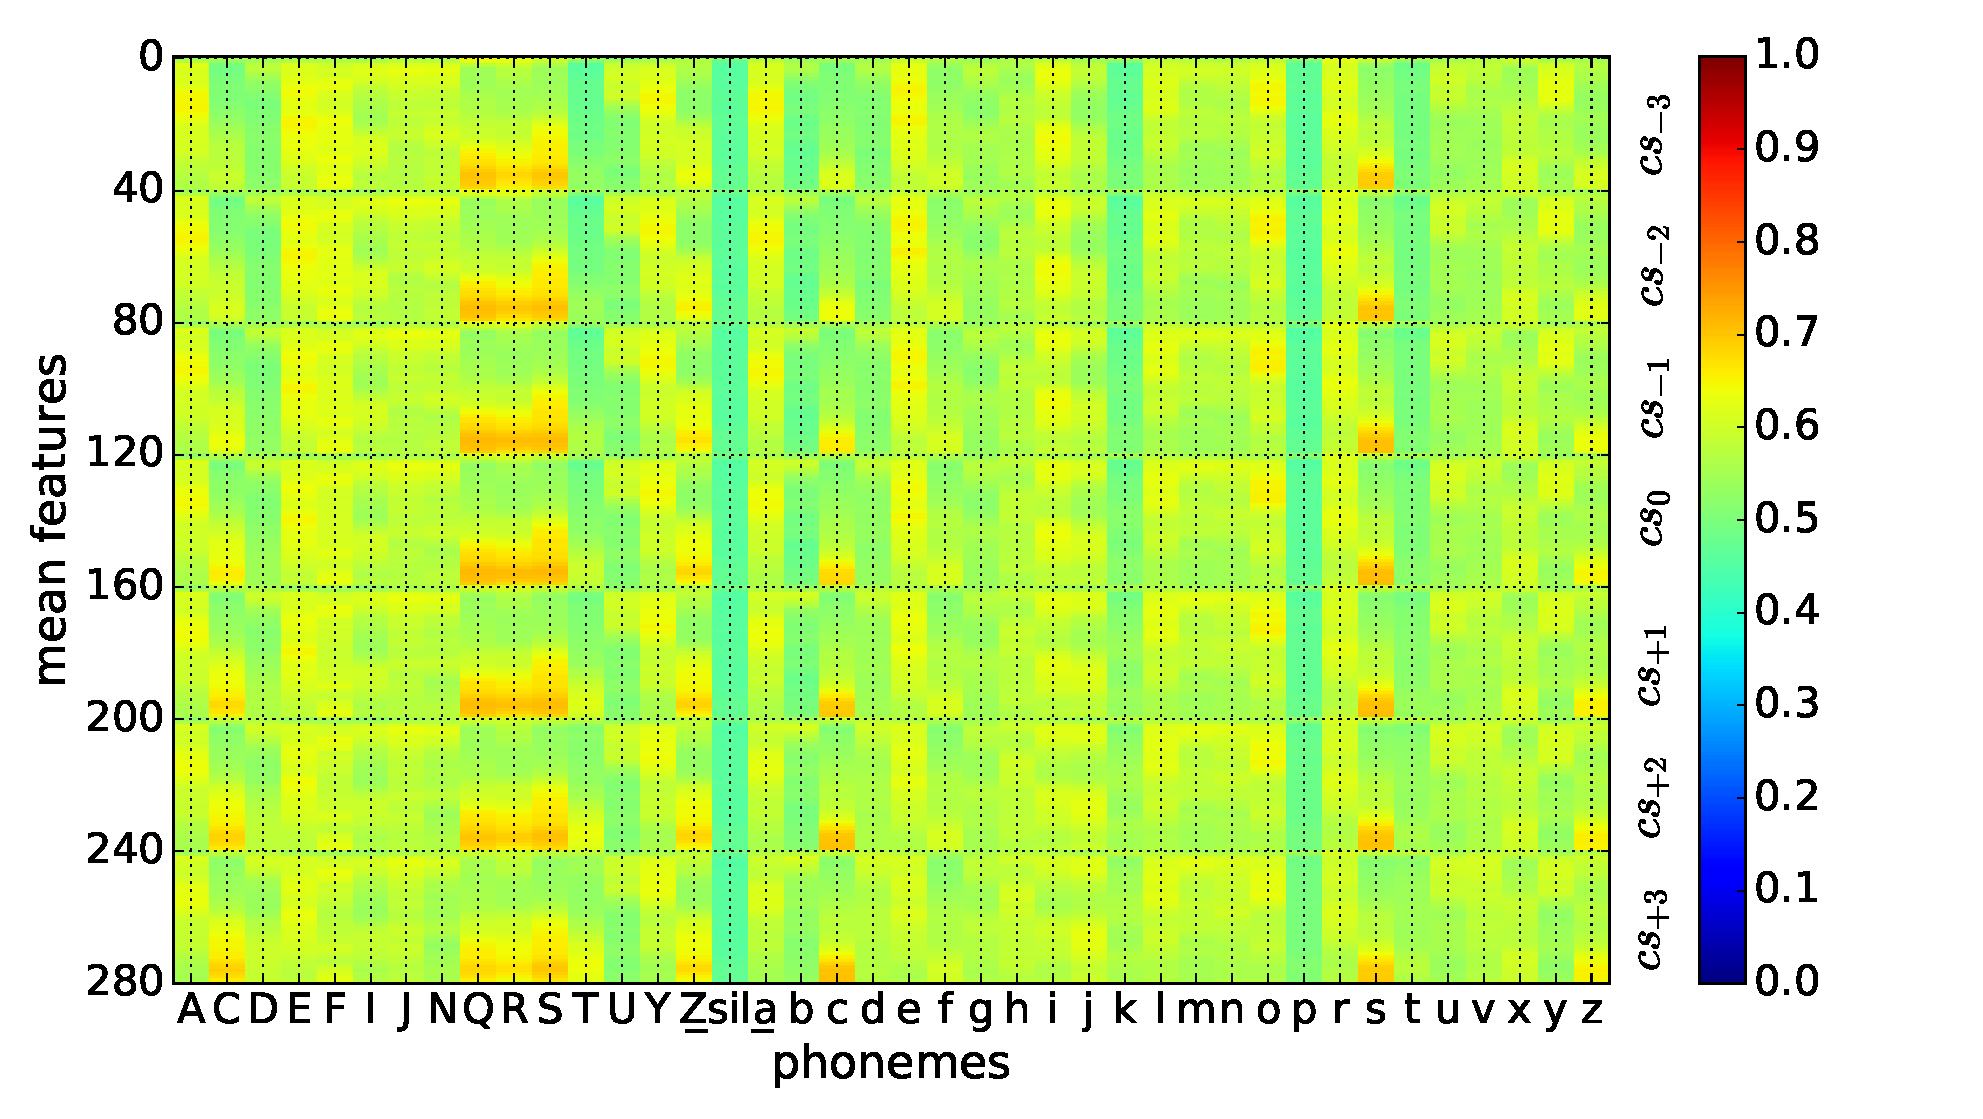
\includegraphics[width=0.8\textwidth]{average_sample_10K_cs3_norm.eps}
\caption{Average sample for each phoneme, $ cs = 3 $.}
\label{fig:app:speech_average_sample_cs3}
\end{figure}

The bottleneck network from \cref{sec:example_speech} was not expected to perform the classification very well. The confusion matrix in \cref{fig:app:speech_bottleneck_cm} confirms this hypothesis. However the goal was to show the representation of selected phonemes in 2D space of the bottleneck layer and we can see that those selected phonemes (e. g. \texttt{"A"}, \texttt{"E"}, \texttt{"S"}, \texttt{"\_sil\_"}, \texttt{"z"} or \texttt{"i"}) turned out quite well compared to the others. 

\begin{figure}[H]
\centering
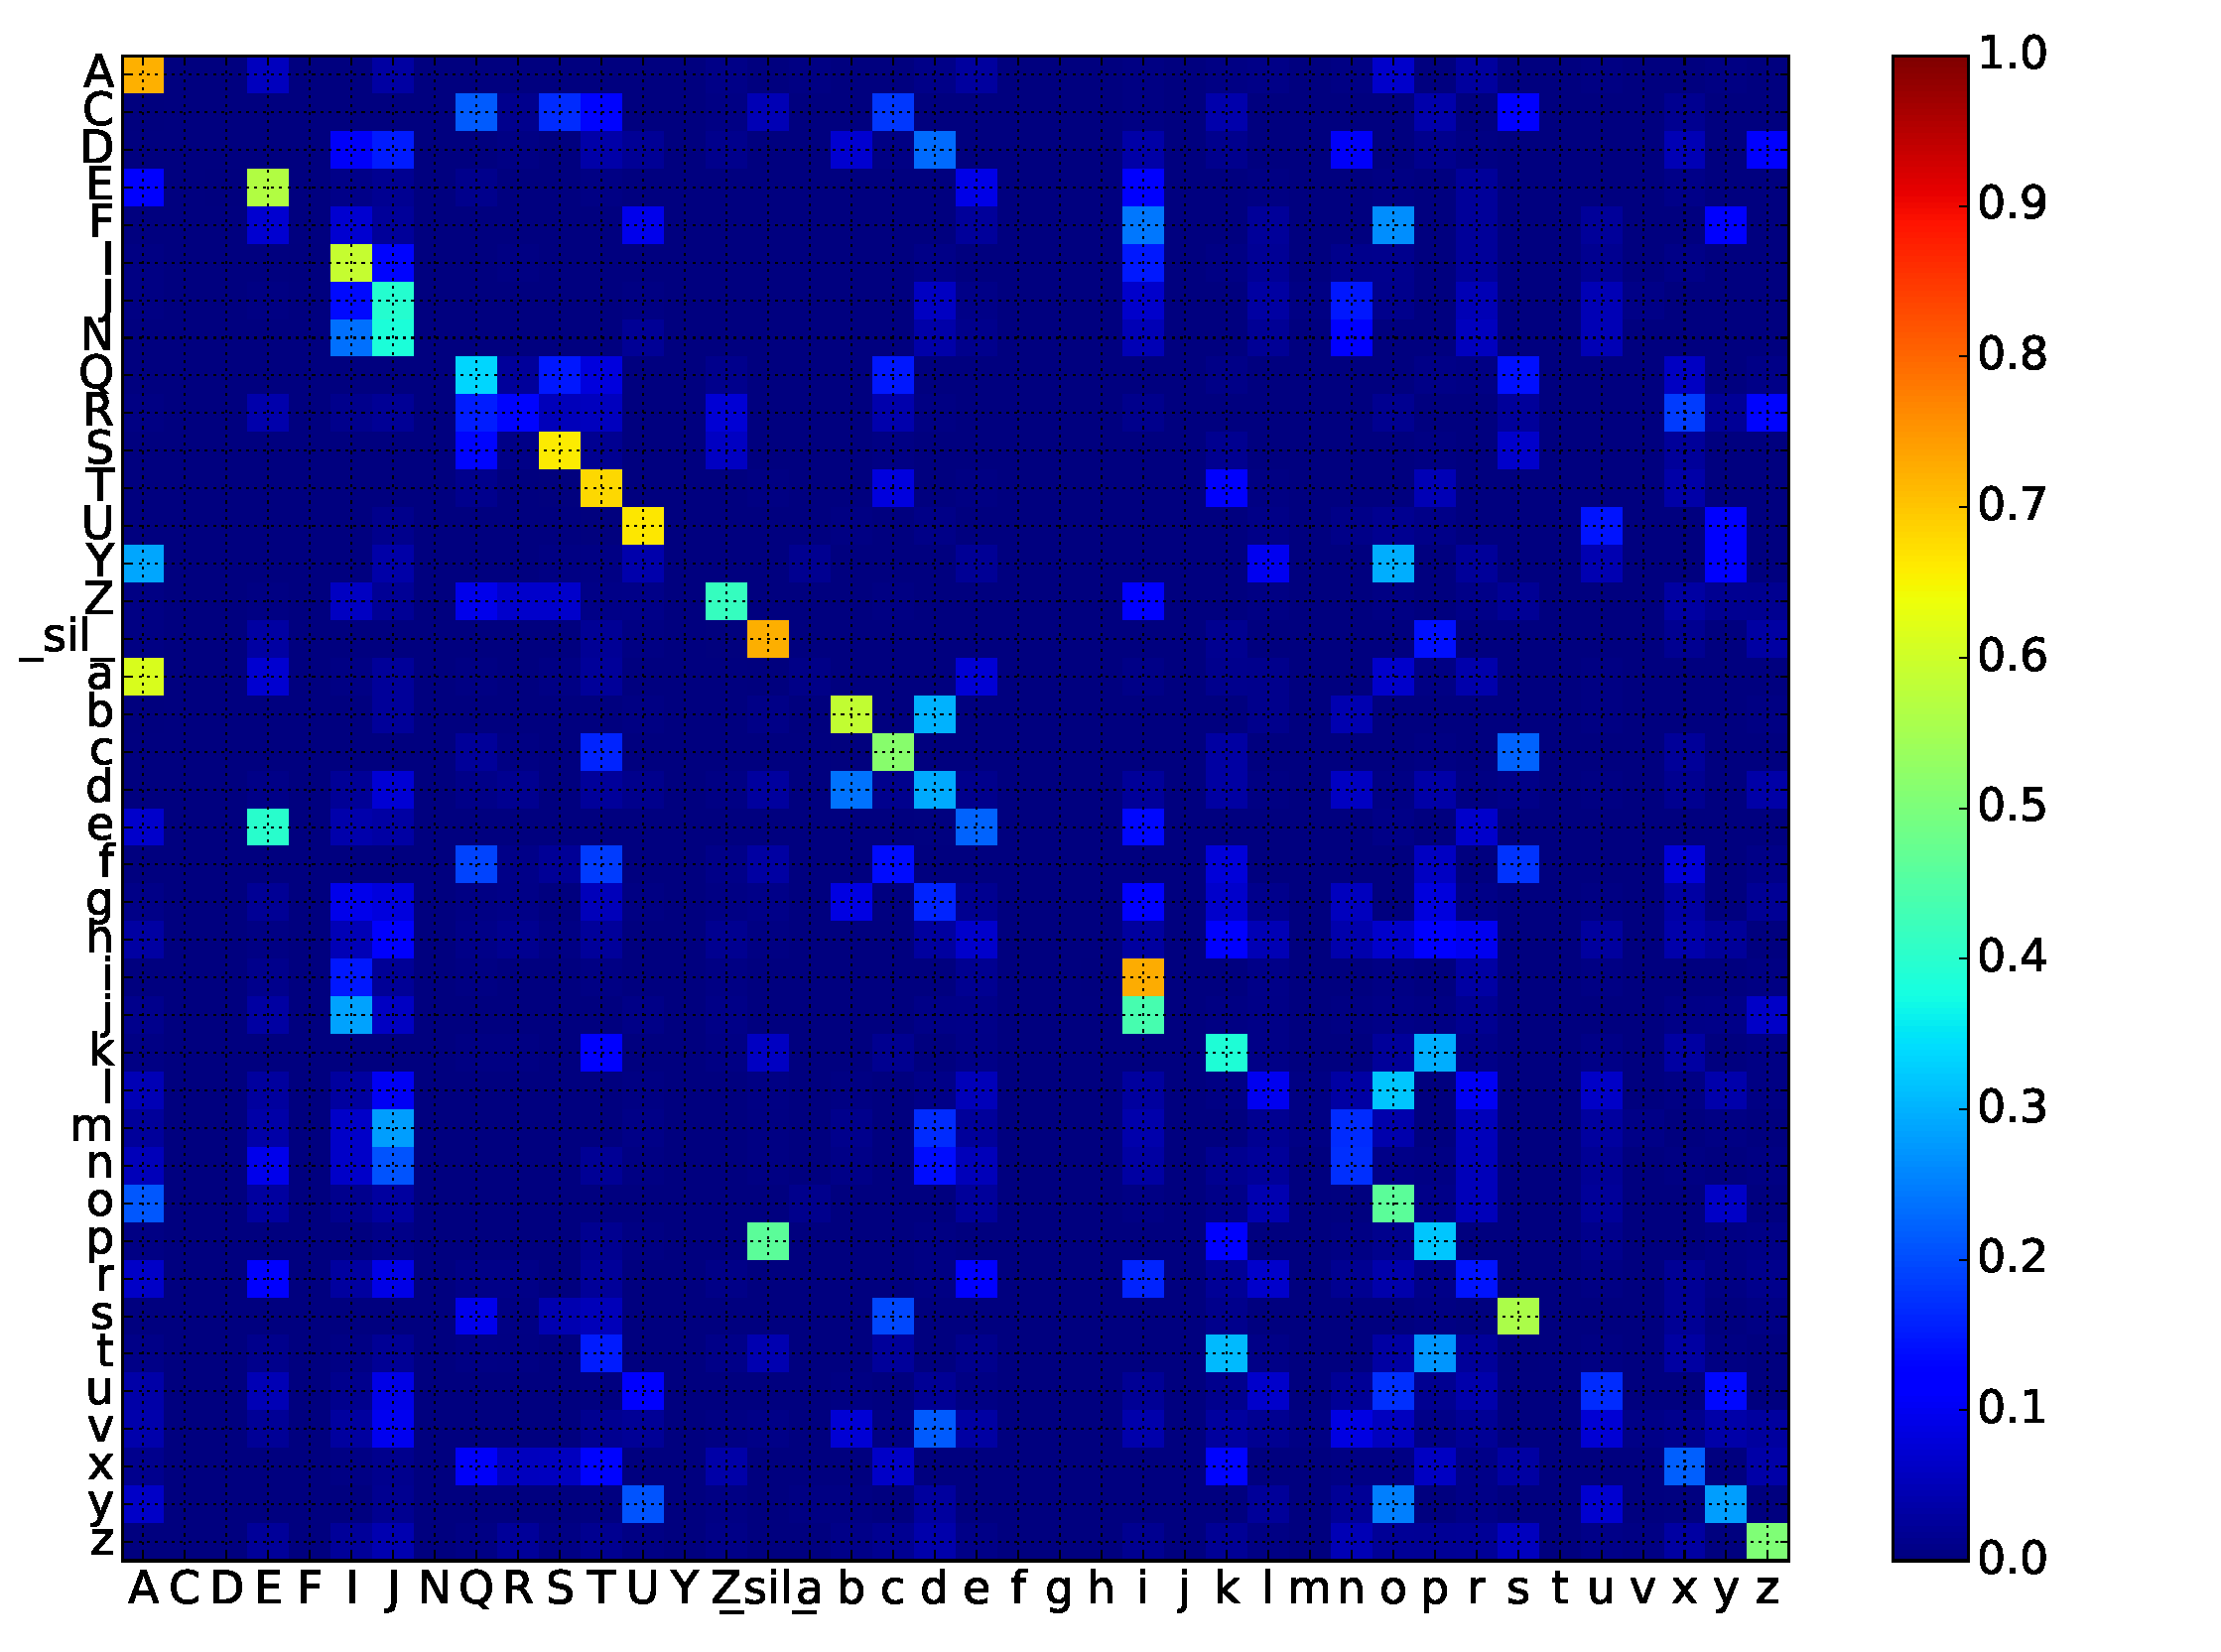
\includegraphics[width=0.7\textwidth]{speech_bottleneck_cm.eps}
\caption{Trained bottleneck network (speech dataset): confusion matrix.}
\label{fig:app:speech_bottleneck_cm}
\end{figure}

\cref{fig:app:speech_fe_set2} shows a set of another 12 phonemes as a supplement to \cref{fig:examples:speech_fe_set1}.
\begin{figure}[H]
\centering
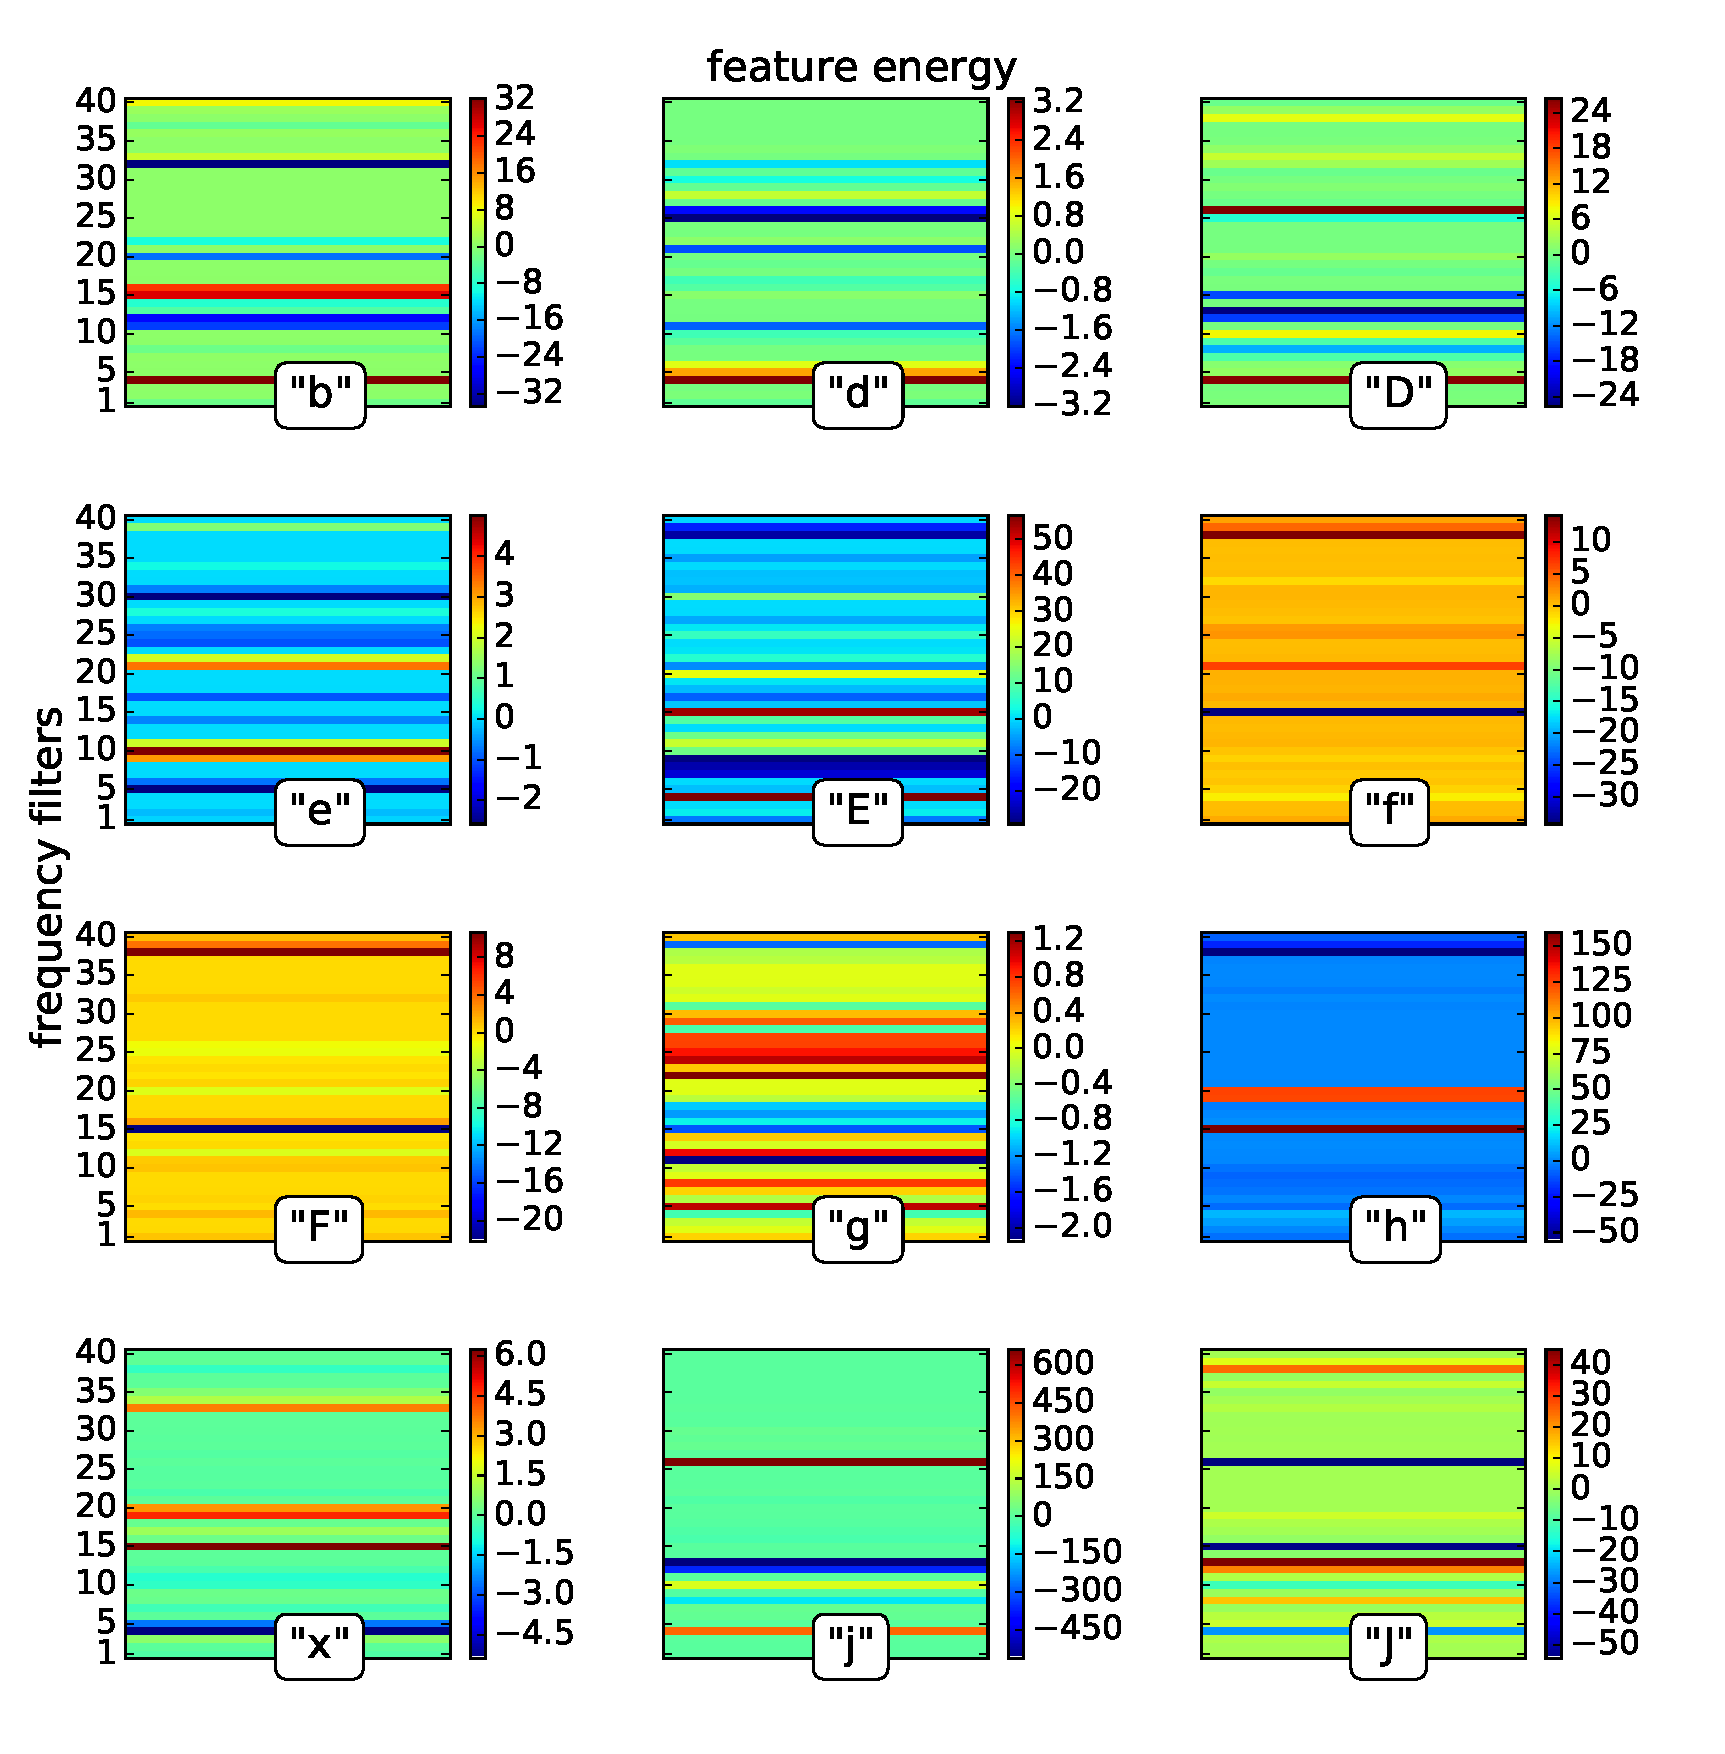
\includegraphics[width=0.8\textwidth]{fe_speech_set2.eps}
\caption{Feature energies for selected phonemes, phoneme set 2.}
\label{fig:app:speech_fe_set2}
\end{figure}

And the rest of the phonemes is illustrated in \cref{fig:app:speech_fe_set3}.

\begin{figure}[H]
\centering
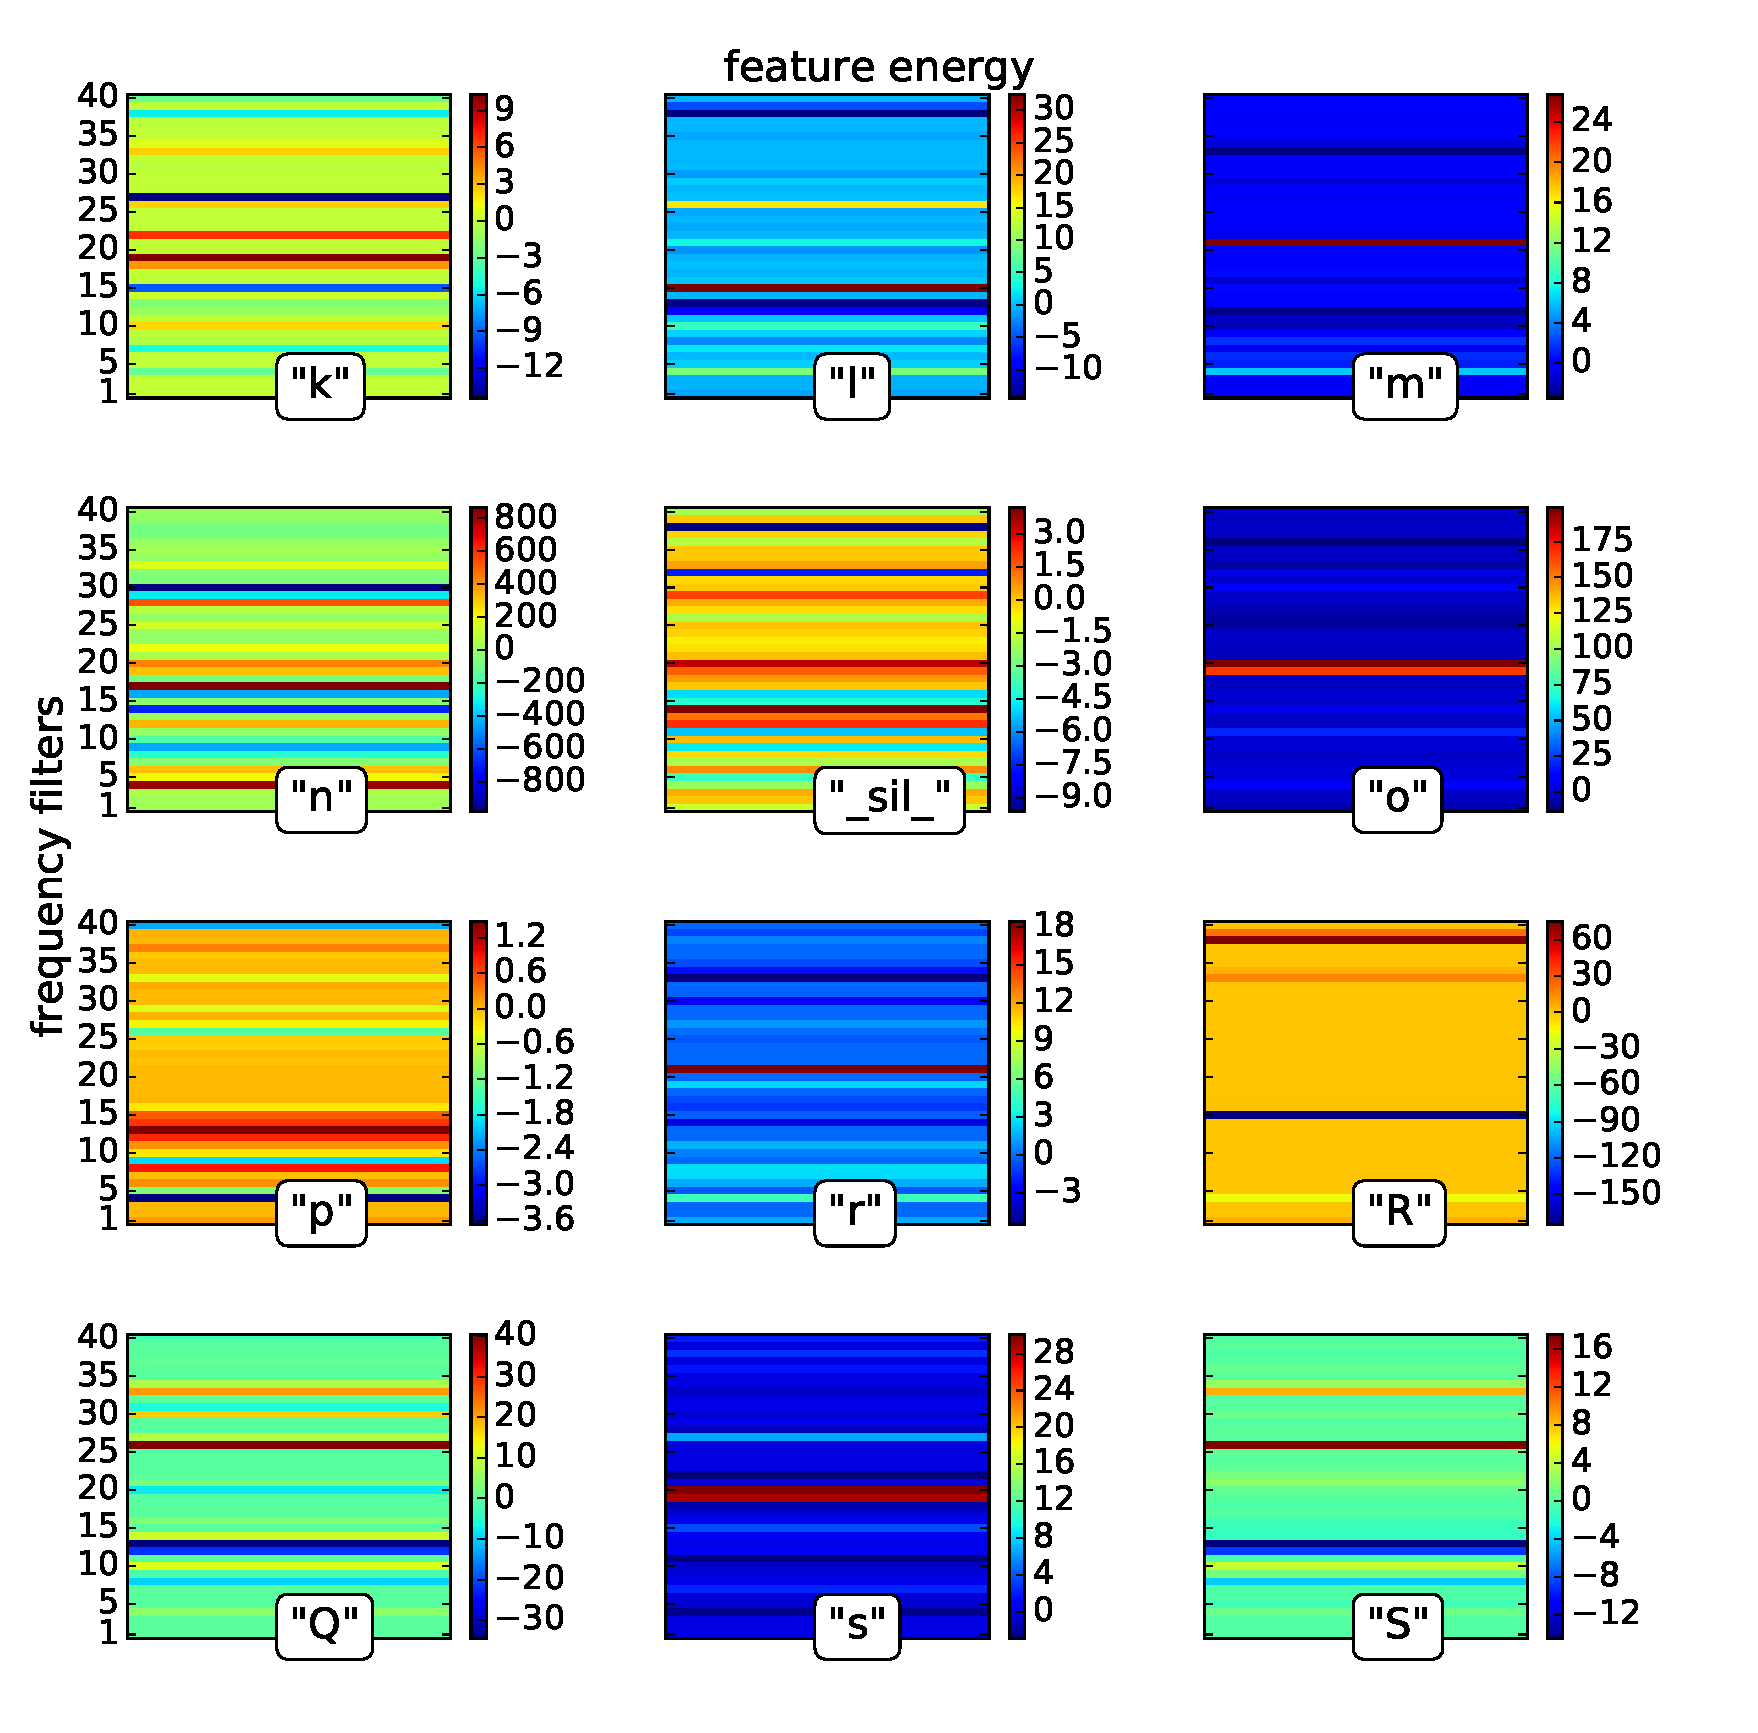
\includegraphics[width=0.9\textwidth]{fe_speech_set3.eps}
\caption{Feature energies for selected phonemes, phoneme set 3.}
\label{fig:app:speech_fe_set3}
\end{figure}

One might note the similarity of \texttt{"o"} and \texttt{"s"} patterns, but remember to check the colorbars. Then we can see that the two phonemes are activated by similar frequencies, but with a different power range. We can also see that \texttt{"S"} and \texttt{"T"} uses a similar power (energy) as well as phonemes \texttt{"p"} and \texttt{"\_sil\_"}.